\subsection{AVL}

\subsubsection{Concept}

An \textbf{AVL Tree} is a \textbf{Binary Search Tree (BST)} that distinguishes itself by being self-balancing. The key characteristic of an AVL tree is that for any node in the tree, the absolute difference between the heights of its left and right subtrees must be at most 1. This difference is known as the \textit{balancing factor}.

Whenever an operation (such as insertion or deletion) causes an imbalance---that is, the balancing factor of a node becomes greater than 1---the tree performs a rebalancing. This process is carried out through specific rotations, which reorganize the nodes to restore the balancing property.

This self-balancing mechanism ensures that operations like insertion, search, and deletion are executed with a time complexity of $O(\log n)$, where $n$ is the number of nodes in the tree. This is crucial for maintaining efficiency, even in trees with a large volume of data. Furthermore, it prevents the degeneration that can occur in a standard BST.


\subsubsection{Implementation}

\begin{itemize}
  \item \underline {\textbf{Function BalancingFactor:}}
  
  In short, the function calculates the balancing factor of a given node by finding the difference between the heights of the right and left subtrees.
  
  \item \underline {\textbf{Function Rotates:}}
  
  As part of the tree's rebalancing, it is necessary to perform rotations on parts of it. Thus, these functions execute rotations in each direction. The transformations performed by each function will be visually represented in the following graphs:

  \begin{itemize}
    \item \textit{\textbf{First Case:}} The node is the root and has no parent.    \begin{center}
    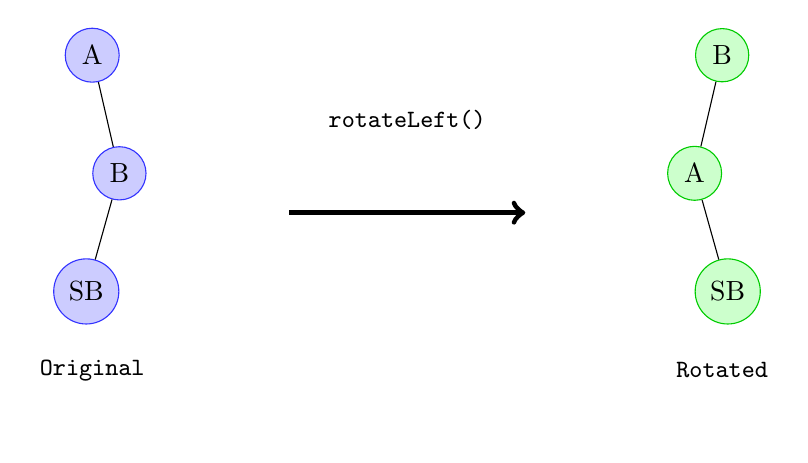
\begin{tikzpicture}[
          level distance=15mm, sibling distance=15mm,
          every node/.style={circle, draw, minimum size=8mm, font=\ttfamily\small}
    ]
    
    \begin{scope}[xshift=-4cm, every node/.style={circle, draw=blue!80, fill=blue!20}]
        \node {A}
            child[right] {node {B}
                child [left]{node {SB}} 
            }
        ;
    \end{scope}
    
    \begin{scope}[xshift=4cm, every node/.style={circle, draw=green!80!black, fill=green!20}]
    \node {B}
      child [left]{node {A}
        child[right] {node {SB}}
      };
    \end{scope}
    
    \draw[->, very thick, line width=2pt] (-1.5,-2.0) -- (1.5,-2.0) 
        node[midway, above, yshift=0.2pt, draw=none, fill=none] {rotateLeft()};
        
    \node[draw=none, fill=none] at (-4, -4) {\textbf{Original} };
    \node[draw=none, fill=none] at (4, -4) {\textbf{Rotated} };
    
    \end{tikzpicture}
    \end{center}

    \item \textit{\textbf{Second Case:}} The node is a left child.  \begin{center}
    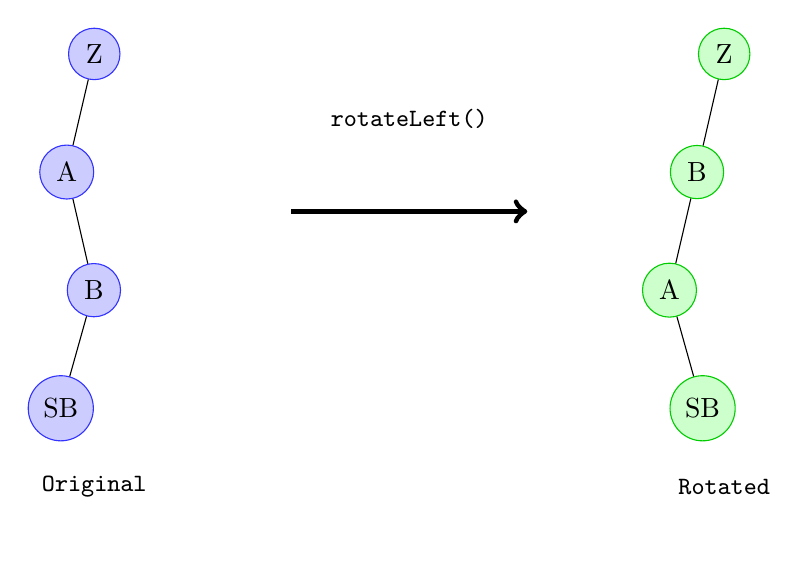
\begin{tikzpicture}[
          level distance=15mm, sibling distance=15mm,
          every node/.style={circle, draw, minimum size=8mm, font=\ttfamily\small}
    ] 
      \begin{scope}[xshift=-4cm, every node/.style={circle, draw=blue!80, fill=blue!20}]
        \node {Z}
          child [left] {
            node {A}
              child [right] {
                node {B}
                  child [left]{node {SB}}
              }
          };

        \end{scope}
        
        \begin{scope}[xshift=4cm, every node/.style={circle, draw=green!80!black, fill=green!20}]
        \node {Z}
          child [left] {
            node {B}
              child [left] {
                node {A}
                  child[right] {node {SB}}
              }
          };

        \end{scope}
        
        \draw[->, very thick, line width=2pt] (-1.5,-2.0) -- (1.5,-2.0) 
            node[midway, above, yshift=0.2pt, draw=none, fill=none] {rotateLeft()};
        
                \node[draw=none, fill=none] at (-4, -5.5) {\textbf{Original} };
        \node[draw=none, fill=none] at (4, -5.5) {\textbf{Rotated} };
        
      \end{tikzpicture}
    \end{center}

      \item \textit{\textbf{Third Case:}} The node is a right child.        
          \begin{center}
    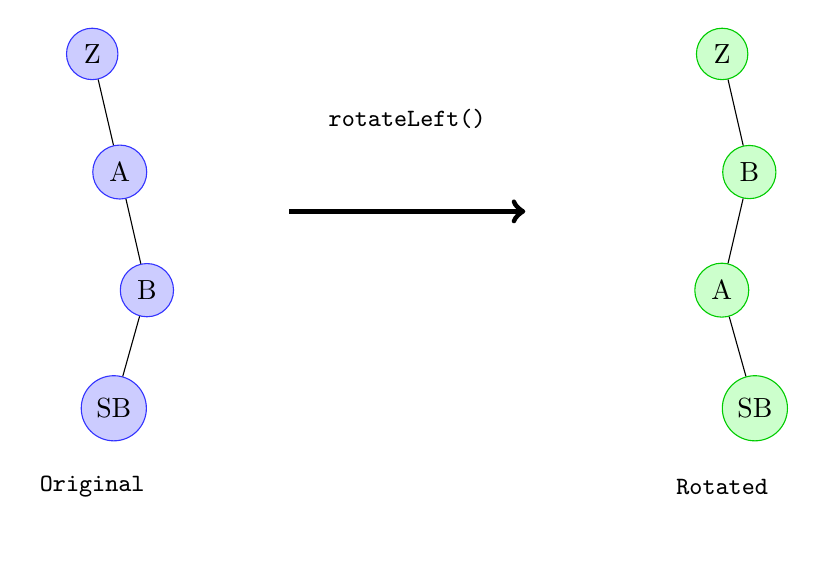
\begin{tikzpicture}[
          level distance=15mm, sibling distance=15mm,
          every node/.style={circle, draw, minimum size=8mm, font=\ttfamily\small}
    ] 
      \begin{scope}[xshift=-4cm, every node/.style={circle, draw=blue!80, fill=blue!20}]
        \node {Z}
          child [right] {
            node {A}
              child [right] {
                node {B}
                  child [left]{node {SB}}
              }
          };

        \end{scope}
        
        \begin{scope}[xshift=4cm, every node/.style={circle, draw=green!80!black, fill=green!20}]
        \node {Z}
          child [right] {
            node {B}
              child [left] {
                node {A}
                  child[right] {node {SB}}
              } 
          };

        \end{scope}
        
        \draw[->, very thick, line width=2pt] (-1.5,-2.0) -- (1.5,-2.0) 
            node[midway, above, yshift=0.2pt, draw=none, fill=none] {rotateLeft()};
        
                \node[draw=none, fill=none] at (-4, -5.5) {\textbf{Original} };
        \node[draw=none, fill=none] at (4, -5.5) {\textbf{Rotated} };
        
      \end{tikzpicture}
    \end{center}

    The rotations presented are derived from the left rotation operation, where the node to be rotated is $A$ and $SB$ represents a subtree. For a right rotation, a similar but mirrored logic is applied. It is important to note that the cases shown do not occur in valid binary search trees, but they constitute the base cases for the rotation algorithms.

    Furthermore, there are what are known as double rotations, which are used when an imbalance occurs at two levels---for example, when a node is a right child, but its own child is a left child (or vice-versa). In these situations, the \texttt{rotateRightLeft} and \texttt{rotateLeftRight} functions are used to restore the tree's balance.

    \item \textit{\textbf{Rotate Left Right:}} Double Rotation
    \begin{center}
    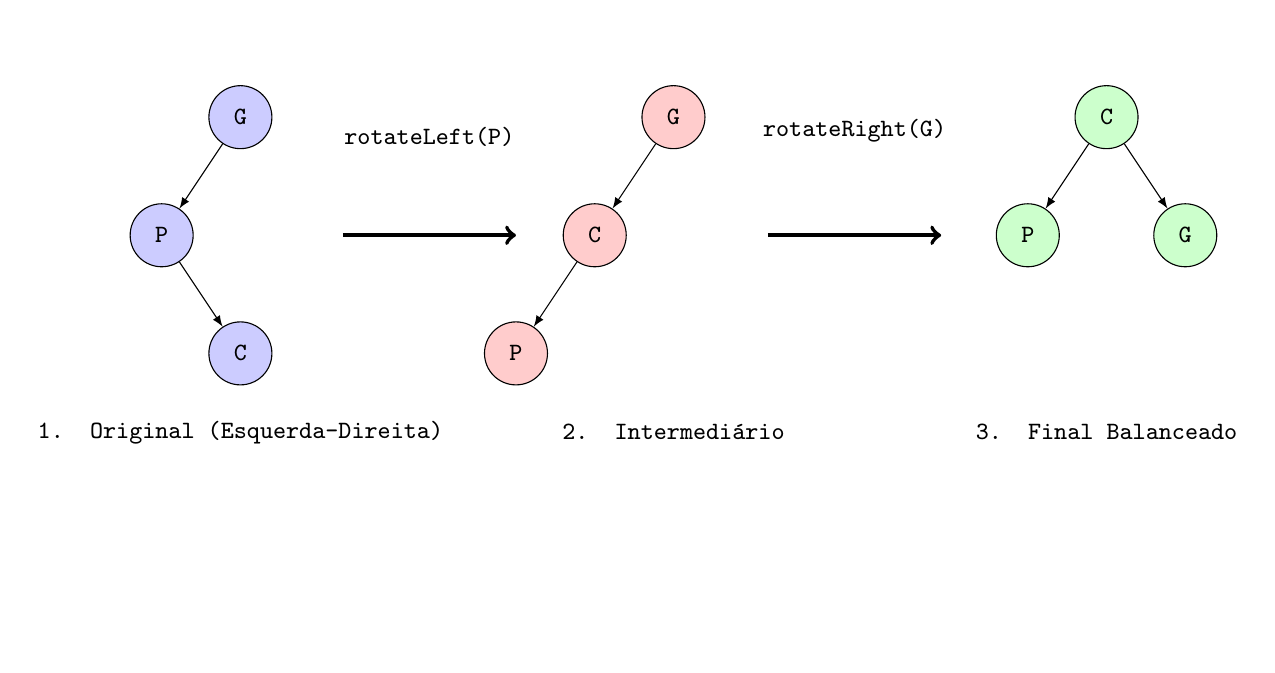
\begin{tikzpicture}[
      level distance=15mm, sibling distance=20mm,
      every node/.style={circle, draw, minimum size=8mm, font=\ttfamily\small},
      edge from parent/.style={draw, -latex}
    ]
    
    \begin{scope}[xshift=-5.5cm]
        \node (G) [fill=blue!20] {G}
            child {node (P) [fill=blue!20] {P}
                child[missing]
                child {node (C) [fill=blue!20] {C}}
            }
            child[missing];
        \node[draw=none, fill=none] at (0, -4) {\textbf{1. Original (Esquerda-Direita)}};
    \end{scope}
    
    \draw[->, very thick, line width=1.5pt] (-4.2cm,-1.5cm) -- (-2cm,-1.5cm) 
        node[midway, above, draw=none, fill=none] {rotateLeft(P)};
    
    \begin{scope}[xshift=0cm]
        \node (G) [fill=red!20] {G}
            child {node (C) [fill=red!20] {C}
                child {node (P) [fill=red!20] {P}}
                child[missing]
            }
            child[missing];
        \node[draw=none, fill=none] at (0, -4) {\textbf{2. Intermediário}};
    \end{scope}
    
    \draw[->, very thick, line width=1.5pt] (1.2cm,-1.5cm) -- (3.4cm,-1.5cm) 
        node[midway, above, draw=none, fill=none] {rotateRight(G)};
    
    \begin{scope}[xshift=5.5cm]
        \node (C) [fill=green!20] {C}
            child {node (P) [fill=green!20] {P}}
            child {node (G) [fill=green!20] {G}};
        \node[draw=none, fill=none] at (0, -4) {\textbf{3. Final Balanceado}};
    \end{scope}
    
    \end{tikzpicture}
    \end{center}
    
  \end{itemize}

  \item \underline{\textbf{Balance Function:}}

  The \texttt{balance} function is responsible for checking if a given node violates the balancing property of an AVL tree. To do this, it first calculates the node's balancing factor. If the absolute value of this factor is greater than 1, it indicates an imbalance and, therefore, the need for a rotation.

  Next, the function determines if the imbalance is in the left or right subtree and checks whether a single or double rotation is needed based on the balancing factor of the corresponding child. After applying the appropriate rotation, the function returns the new, balanced node.

  \item \underline{\textbf{Insert Function:}}

  In general, insertion into an AVL tree follows the same logic as insertion into a BST, divided into two cases: the word is already in the tree, or it is a new entry. After this check, the balancing process begins.

  If the word does not yet exist in the tree, after its insertion as a child of a leaf node, a recursive check is performed from the new node's parent up to the root. At each step, it verifies if the current node maintains the AVL balancing property. If the tree remains balanced, no action is necessary; otherwise, the \texttt{balance} function is called to restore the local balance.

  This process ensures that, by the end of the insertion, all nodes above the new element---all the way to the root---are also balanced. In this way, the entire tree structure continues to adhere to the AVL balancing rules, maintaining its efficiency for search, insertion, and deletion operations.

\end{itemize}













